\subsection{Temperature Targets}\label{temptargets}
The WACCM simulations use the feedback algorithm to maintain three temperature targets in their SAI scenario. These temperature targets are defined in \textcite{kravitz2016} as the projection of $T(\psi)$ onto the first three components of the Legendre polynomial expansion of $\sin(\psi)$,

\begin{equation}\label{eq:Tpsi}
    \begin{split}
        T_0 &= \frac{1}{2} \int\displaylimits_{-\pi/2}^{\pi/2} T(\psi) \cos(\psi) \mathop{d\psi},\\
        T_1 &= \frac{1}{2} \int\displaylimits_{-\pi/2}^{\pi/2} T(\psi) \sin(\psi) \cos(\psi) \mathop{d\psi},\\
        T_2 &= \frac{1}{2} \int\displaylimits_{-\pi/2}^{\pi/2} T(\psi) \frac{1}{2}(2\sin^2(\psi) -1) \cos(\psi) \mathop{d\psi},
    \end{split}
\end{equation}

\noindent where $\psi$ is latitude, $T(\psi)$ is the zonal-mean temperature for each latitude.

The $T_0$ temperature target translates to global mean surface temperature (GMST), the $T_1$ is interpreted as the inter-hemispheric temperature gradient and $T_2$ is interpreted as the equator-to-pole temperature gradient. From the model output these temperature targets can be evaluated using Eq. \ref{eq:Tpsi}. 


\subsection{Using the CESM2(CAM6) Emulator for SAI simulations}\label{emulator_pt1}
The emulator for SAI simulations is introduced in \textcite{pfluger2024}, it implements SAI via prescribed aerosol fields, as opposed to sulphate injections that result in aerosol fields through model physics. As per \textcite{pfluger2024}, the protocol works as follows:
\begin{itemize}
    \item Every year, observe the deviation of GMST from the target.
    \item Based on past GMST deviations, infer the level of SAI - expressed in terms of global mean aerosol optical depth (AOD) - which is necessary to achieve the desired target.
    \item Use the AOD to scale all SAI-related aerosol fields appropriately.
    \item Feed the scaled fields into CAM6.
\end{itemize}

The first two steps are implemented via the feedforward-feedback control algorithm as established in \textcite{kravitz2017}. The control algorithm stabilises only GMST, not inter-hemispheric and equator-to-pole temperature gradients from section \ref{temptargets}.

The prescribed aerosol fields are the averaged aerosol fields from the WACCM simulation, this simulation is called the \textit{Geo SSP5-8.5 1.5 scenario} in \textcite{tilmes2020}. The fields are normalised, averaged and fit, to then arrive at an amplitude for each aersol component. The SO$_4$ concentration from WACCM in 2100 at each latitude and model layer is shown in Figure \ref{fig:strataero}. The highest concentration of aerosols is found around the four injection points, concentrations are lower toward the poles. There are also higher concentrations in the Southern Hemisphere than in the Northern Hemisphere.

\begin{figure}[H]
	\centering
	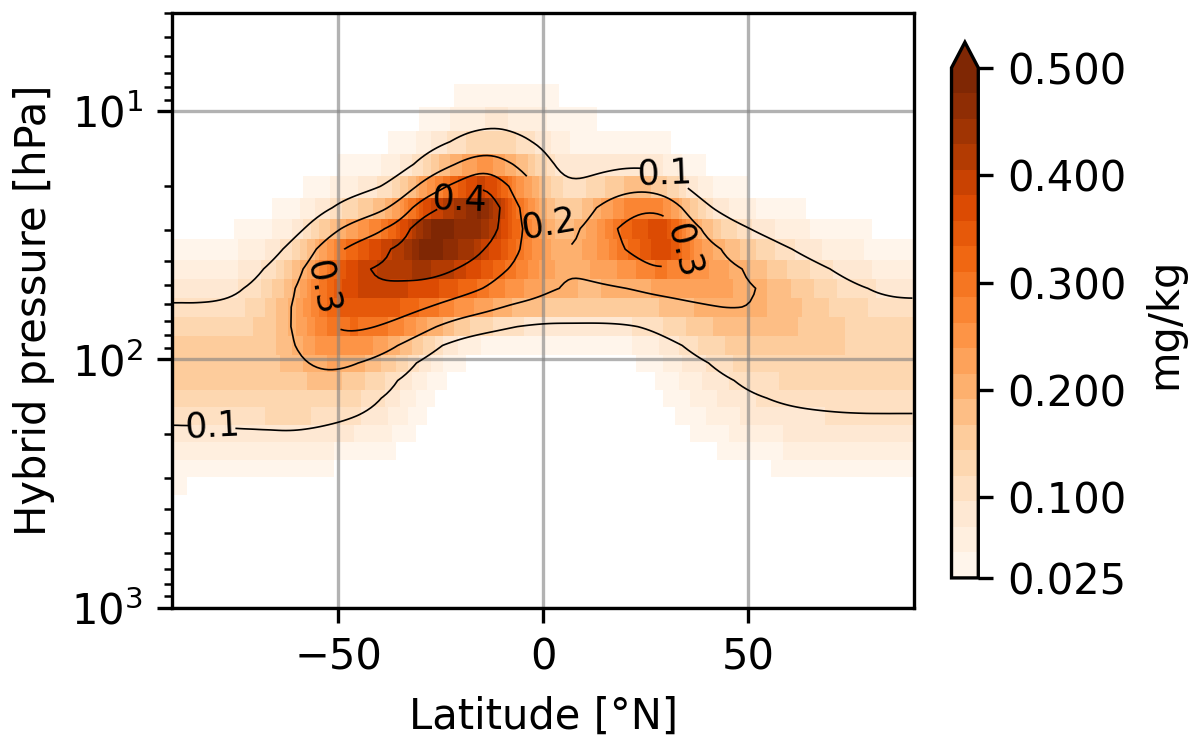
\includegraphics[width=0.6\linewidth]{images/strataero.png}
	\caption{Total SO$_4$ concentration from WACCM in 2100.}
	\label{fig:strataero}
\end{figure}

\subsection{Definition of Scenarios and Time Periods for Part I}
There are two simulations performed with each CESM2 configuration. The first simulation follows the historical spin-up and is continued by the SSP5-8.5 scenario. The second simulation branches from the first simulation in 2020 and from then on introduces SAI to stabilise temperatures using the SSP5-8.5 scenario as background. Here we will refer to it as the gradual SAI scenario. 

Throughout this first part, three time periods are selected to visualise and interpret the results from the simulations. For each period the 20-year mean is taken, unless specified otherwise. These periods are defined as follows:

\begin{itemize}
    \item \textbf{Reference} The period 2016-2035 of the SSP5-8.5 simulation.
    \item \textbf{Control} The period 2080-2099 of the SSP5-8.5 simulation.
    \item \textbf{SAI 2020} The period 2080-2099 of the gradual SAI simulation.
\end{itemize} %tabel van maken


\subsection{Vertical Interpolation}
The atmospheric vertical levels of CESM are defined at hybrid pressure coordinates. However, for ease of computation and visualisation, conversion to pressure coordinates is preferred. The hybrid pressure coordinates are converted to pressure coordinates for each timestep at each gridpoint. Then a logarithmic interpolation scheme is used to project the model output onto uniform constant pressure coordinates. For a variable $f$ at pressure coordinate $p$ the scheme takes the form

\begin{equation}
    f = \frac{f_1 - f_0}{\ln\frac{p_1}{p_0}} \cdot \ln \frac{p}{p_1} + f_0.
\end{equation}

For CAM the model output is converted to 34 pressure levels ranging from 3.5 to 993 hPa. We add two levels in the upper stratosphere, compared to the model output, for ease of analysis of patterns. For WACCM the SSP5-8.5 model output was pubplished in pressure levels, 19 pressure levels ranging from 1 to 1000 hPa. The WACCM gradual SAI scenario model output is converted to those same 19 pressure levels to enable direct comparison.

No interpolation is needed of the horizontal grids as these are identical in all models. 


\subsection{Potential Temperature}
With the vertical coordinate converted to pressure coordinates, the potential temperature $\theta$ is calculated through
\begin{equation}
    \theta = T\left( \frac{p_{ref}}{p} \right)^\kappa, 
\end{equation}
where $T$ is the air temperature, $p_{ref} = 1000$ hPa is the reference pressure, $p$ is the pressure. $\kappa$ is the ratio $\frac{c_p - c_v}{c_p}$, with $c_p = 1004$ J kg$^{-1}$ K$^{-1}$ the specific heat of an ideal gas at constant pressure and $c_v = 717$ J kg$^{-1}$ K$^{-1}$ that at constant volume. 
